%刚体的绕轴转动 转动惯量

\pentry{刚体\upref{RigBd}, 角动量定理\upref{AMLaw}}

设刚体绕光滑轴转动.这里令轴的方向为 $z$,假设轴光滑,则轴对刚体可施加 $x, y$ 两个方向的力矩,却不能施加 $z$ 方向的力矩. 所以根据角动量定理, 角动量 $\vec L$ 的 $z$ 分量 $L_z$ 守恒. 我们下面来推导 $L_z$ 与角速度 $\omega$ 的关系. 矢量 $\vec L$ 与矢量 $\vec omega$ 的关系见角动量张量\upref{ITensr}.

对于单个质点,$L_z = ( \vec r \cross \vec p ) \vdot \uvec z$. 首先把质点的位矢在水平方向和竖直方向分解, $\vec r = \vec r_z + \vec r_ \bot$. 由于 $\vec p$ 一直沿水平方向, 根据叉乘的几何定义, $\vec r_z \cross \vec p$ 也是沿水平方向, 只有 $\vec r_ \bot \cross \vec p$ 沿 $z$ 方向.另外, 在圆周运动中, 半径始终与速度垂直, 所以 $\vec r_ \bot$ 始终与 $\vec p$ 垂直.得出结论
\begin{equation}
L_z = \abs{\vec r_\bot} \abs{\vec p} = m r_ \bot v = mr_ \bot ^2\omega 
\end{equation}
若把刚体分成无数小块, 每小块的质量分别为 $m_i$, 离轴的距离 $r_{\bot i} = \sqrt{x_i^2 + y_i^2} $, 则刚体的角动量 $z$ 分量为
\begin{equation}
L_z = \omega \sum_i m_i r_{ \bot i}^2
\end{equation}
用积分写成
\begin{equation}
L_z = \omega \int r_ \bot ^2 \dd{m} = \omega \int r_ \bot ^2\rho  \dd{V} 
\end{equation}

定义刚体的\bb{绕轴转动惯量}为
\begin{equation}
I = \int r_ \bot ^2 \dd{m} 
\end{equation}
(注意角动量的大小不仅取决于刚体的质量分布, 还取决于转轴的位置和方向)则刚体沿轴方向的角动量为
\begin{equation}\label{RigRot_eq5}
L_z = I\omega 
\end{equation}
 
现在来看“角动量定理\upref{AMLaw}” 的\autoref{AMLaw_eq1}, 注意等号两边是矢量, 所以各个分量必须相等, 我们有
\begin{equation}\label{RigRot_eq6}
\dv{L_z}{t} = M_z
\end{equation}
将\autoref{RigRot_eq5} 代入\autoref{RigRot_eq6}, 并利用角加速度的定义得
\begin{equation}\label{RigRot_eq7}
I\alpha = M_z
\end{equation}
这就是刚体绕轴转动的动力学方程, 其形式可类比牛顿第二定律\upref{New3}.

\begin{exam}{刚体摆}\label{RigRot_ex1}
如\autoref{RigRot_fig1}, 已知质量为 $M$ 的薄片绕某点的转动惯量为 $I$, 转轴到刚体质心的长度为 $r_c$, 转轴和质心的连线与竖直方向夹角为 $\theta$, 求刚体的运动方程.
\begin{figure}[ht]
\centering
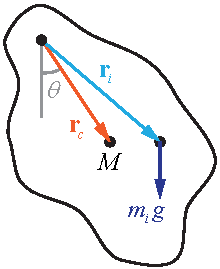
\includegraphics[width=3.8cm]{./figures/RigRot1.pdf}
\caption{刚体摆} \label{RigRot_fig1}
\end{figure}

首先我们把刚体看做质点系, 以转轴为原点计算刚体的合力矩为(由于这是一个平面问题, 力矩必然垂直于该平面)
\begin{equation}\ali{
\vec M &= \sum_i \vec r_i \cross (m_i \vec g)
= \qty(\sum_i m_i \vec r_i) \cross \vec g
= M \vec r_c \cross \vec g\\
&= Mg r_c \sin\theta
}\end{equation}
这就说明, 刚体所受力矩相当于质量为 $M$, 长度为 $r_c$ 的单摆所受的力矩. 代入\autoref{RigRot_eq7} 得刚体摆的运动方程为
\begin{equation}
I\ddot \theta = Mg r_c \sin\theta
\end{equation}
可以验证当刚体的质量全部集中在质心时($I = Mr_c^2$)我们就得到了单摆的运动方程\autoref{Pend_eq4}\upref{Pend}.
\end{exam}

\begin{exer}{陀螺进动的角速度}
在“角动量定理\upref{AMLaw}” 的\autoref{AMLaw_ex2} 中, 如果除 $r_0, m, g$ 外, 还知道陀螺的转动惯量为 $I$ 和陀螺的角速度 $\omega$, 试证明陀螺进动的角速度为
\begin{equation}
\Omega = \frac{mgr_0}{I\omega}
\end{equation}
注意进动角速度与陀螺倾角 $\theta$ 无关.
\end{exer}










